% Generated by scripts/make_explanation_figures.py from experiment_0013 (do not edit by hand).
% Model: COVER
\documentclass[tikz,border=3pt]{standalone}
\usepackage[T1]{fontenc}
\usepackage[utf8]{inputenc}
\usepackage{newtxtext,newtxmath}
\usetikzlibrary{positioning,arrows.meta,calc}

\definecolor{neural}{HTML}{2F6DB5}
\definecolor{neuralbg}{HTML}{E8F0FA}
\definecolor{logic}{HTML}{2E8B57}
\definecolor{logicbg}{HTML}{E6F4EC}
\definecolor{relneg}{HTML}{C0392B}

\tikzset{
  tok/.style={draw=neural!80, fill=white, rounded corners=1.5pt, inner sep=1.6pt, font=\scriptsize,
              minimum height=4mm, anchor=base},
  htok/.style={tok, fill=neural!12},
  stok/.style={tok, draw=black!25, text=black!45},
  aedge/.style={line width=#1, draw=logic},
  cedge/.style={line width=#1, draw=relneg},
  ledge/.style={line width=#1, draw=neural, densely dashed},
  rlab/.style={font=\tiny, fill=white, inner sep=0.6pt},
}
\newcommand{\bars}[4]{%
  \fill[logic]  (#1-0.17,0.05) rectangle ++(0.15,{0.8*#2});
  \fill[relneg] (#1+0.02,0.05) rectangle ++(0.15,{0.8*#3});
  \node[font=\tiny, anchor=north] at (#1-0.095,0.03) {$s$};
  \node[font=\tiny, anchor=north] at (#1+0.095,0.03) {$c$};
  \node[font=\tiny, anchor=north] at (#1,-0.22) {$#2\,/\,#3$};
  \node[font=\tiny, anchor=north, text=black!60] at (#1,-0.47) {$\omega{=}#4$};
}
\newcommand{\sbar}[3]{%
  \fill[logic]  (#1-0.075,0.05) rectangle ++(0.15,{0.8*#2});
  \node[font=\tiny, anchor=north] at (#1,0.03) {$s$};
  \node[font=\tiny, anchor=north] at (#1,-0.22) {$#2$};
  \node[font=\tiny, anchor=north, text=black!60] at (#1,-0.47) {$\omega{=}#3$};
}
\providecommand{\Pcov}{P_{\mathrm{cov}}}
\providecommand{\Pnc}{P_{\neg\mathrm{conf}}}
\providecommand{\E}{\textsc{e}}
\providecommand{\N}{\textsc{n}}
\providecommand{\C}{\textsc{c}}

\begin{document}
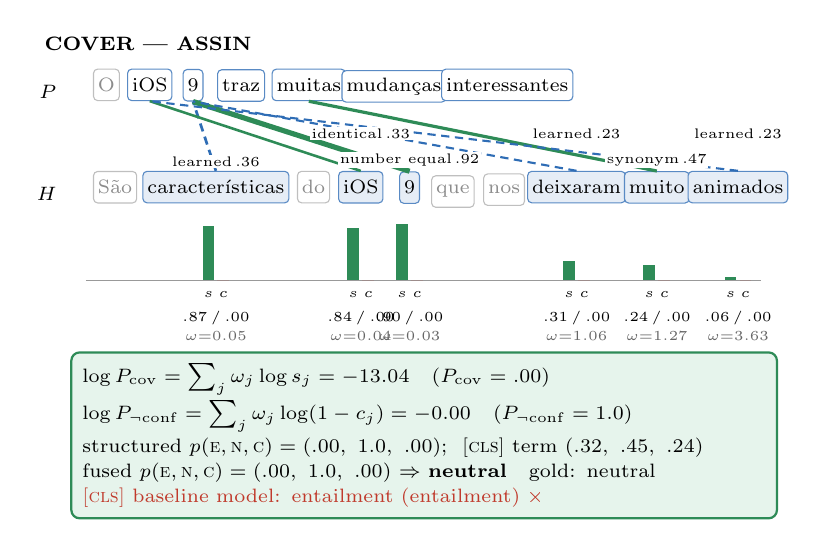
\begin{tikzpicture}
\node[font=\scriptsize\itshape, anchor=east] at (-0.35,2.45) {$P$};
\node[font=\scriptsize\itshape, anchor=east] at (-0.35,1.15) {$H$};
\node[stok] (pw0) at (0.16,2.45) {O};
\node[tok] (p2) at (0.71,2.45) {iOS};
\node[tok] (p4) at (1.26,2.45) {9};
\node[tok] (p5) at (1.87,2.45) {traz};
\node[tok] (p6) at (2.73,2.45) {muitas};
\node[tok] (p7) at (3.81,2.45) {mudanças};
\node[tok] (p8) at (5.25,2.45) {interessantes};
\node[stok] (hw0) at (0.27,1.15) {São};
\node[htok] (h12) at (1.55,1.15) {características};
\node[stok] (hw2) at (2.79,1.15) {do};
\node[htok] (h14) at (3.39,1.15) {iOS};
\node[htok] (h16) at (4.01,1.15) {9};
\node[stok] (hw5) at (4.56,1.15) {que};
\node[stok] (hw6) at (5.21,1.15) {nos};
\node[htok] (h19) at (6.13,1.15) {deixaram};
\node[htok] (h20) at (7.15,1.15) {muito};
\node[htok] (h21) at (8.18,1.15) {animados};
\draw[ledge=0.98pt] (h12.north) -- (p4.south);
\draw[aedge=0.93pt] (h14.north) -- (p2.south);
\draw[aedge=1.87pt] (h16.north) -- (p4.south);
\draw[ledge=0.77pt] (h19.north) -- (p4.south);
\draw[aedge=1.15pt] (h20.north) -- (p6.south);
\draw[ledge=0.76pt] (h21.north) -- (p2.south);
\node[rlab, anchor=south] at (1.55,1.47) {learned\,.36};
\node[rlab, anchor=south] at (3.39,1.83) {identical\,.33};
\node[rlab, anchor=south] at (4.01,1.47) {number equal\,.92};
\node[rlab, anchor=south] at (6.13,1.83) {learned\,.23};
\node[rlab, anchor=south] at (7.15,1.47) {synonym\,.47};
\node[rlab, anchor=south] at (8.18,1.83) {learned\,.23};
\draw[black!40] (-0.1,0.05) -- (8.47,0.05);
\bars{1.55}{.87}{.00}{0.05}
\bars{3.39}{.84}{.00}{0.04}
\bars{4.01}{.90}{.00}{0.03}
\bars{6.13}{.31}{.00}{1.06}
\bars{7.15}{.24}{.00}{1.27}
\bars{8.18}{.06}{.00}{3.63}
\node[draw=logic, fill=logicbg, rounded corners=3pt, line width=0.8pt, font=\scriptsize, align=left, anchor=north west, text width=8.68cm, inner sep=4pt] (agg) at (-0.3,-0.85) {%
  $\log\Pcov=\sum_j\omega_j\log s_j=-13.04$\quad($\Pcov=.00$)\\[1pt]$\log\Pnc=\sum_j\omega_j\log(1-c_j)=-0.00$\quad($\Pnc=1.0$)\\[1pt]structured $p(\E,\N,\C)=(.00,\ 1.0,\ .00)$;\ \ \textsc{[cls]} term $(.32,\ .45,\ .24)$\\[1pt]fused $p(\E,\N,\C)=(.00,\ 1.0,\ .00)$ $\Rightarrow$ \textbf{neutral}\quad gold: neutral\\[1pt]\textcolor{relneg}{\textsc{[cls]} baseline model: entailment (entailment) \texttimes}};
\node[font=\scriptsize\bfseries, anchor=south west] at (-0.75,2.85) {COVER --- ASSIN};
\end{tikzpicture}
\end{document}
